\documentclass[tikz,border=10pt]{standalone}
%\documentclass{article}

\usepackage{tikz}
\usepackage[charter]{mathdesign}
\usepackage[none]{hyphenat}
\usetikzlibrary{shapes.geometric, arrows, positioning, trees, fit, chains,matrix,calc,arrows.meta,decorations,calligraphy}

\begin{document}
\begin{figure}
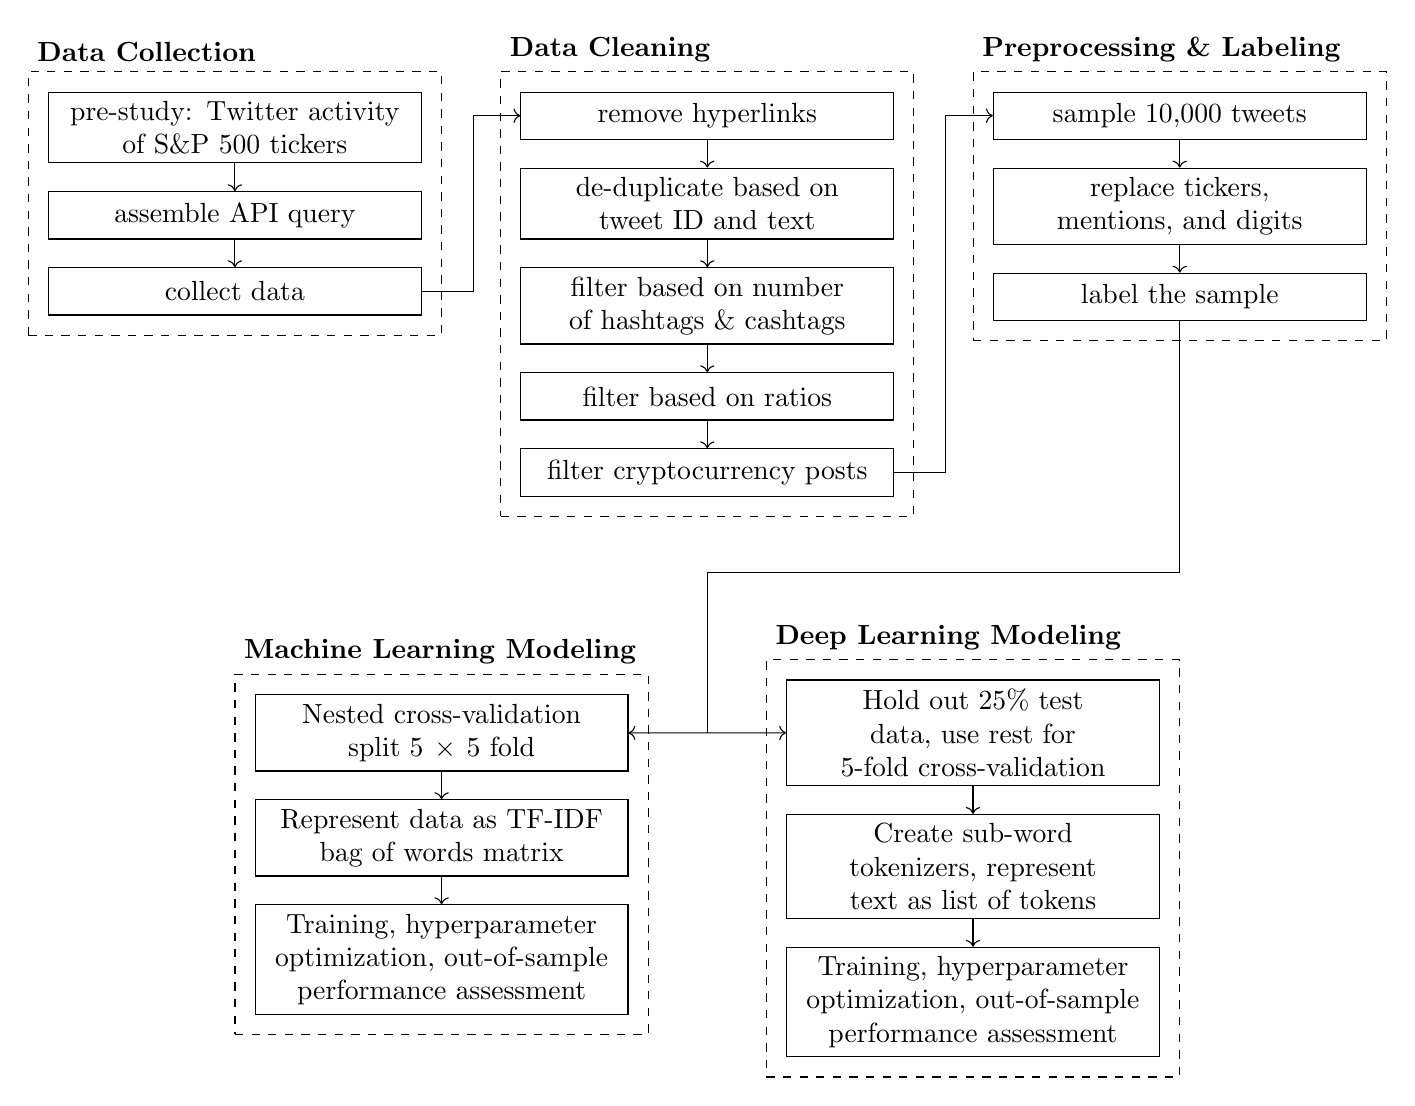
\begin{tikzpicture}


\tikzstyle{mynode}=[draw,text width=4.5cm, minimum height=0.6cm,align=center]

% NODES
% data collection
\node[mynode](ps){pre-study: Twitter activity of S\&P 500 tickers};
\node[mynode, below=1em of ps](qu){assemble API query};
\node[mynode, below=1em of qu](coll){collect data};

% cleaning
\node[mynode, right=6cm of ps.north,anchor=north](hyp){remove hyperlinks};
\node[mynode, below=1em of hyp](dedupe){de-duplicate based on tweet ID and text};
\node[mynode, below=1em of dedupe](nct){filter based on number of hashtags \& cashtags};
\node[mynode, below=1em of nct](ratio){filter based on ratios};
\node[mynode, below=1em of ratio](crypto){filter cryptocurrency posts};

% labeling & prep
\node[mynode, right=6cm of hyp.north,anchor=north](sample){sample 10,000 tweets};
\node[mynode, below=1em of sample](prettify){replace tickers, mentions, and digits};
\node[mynode, below=1em of prettify](annot){label the sample};

% ARROWS
\draw[->](ps) -- (qu);
\draw[->](qu) -- (coll);

\draw[->](coll.east) -| ([xshift=-0.6cm]hyp.west) -- (hyp.west);
\draw[->](hyp) -- (dedupe);
\draw[->](dedupe) -- (nct);
\draw[->](nct) -- (ratio);
\draw[->](ratio) -- (crypto);

\draw[->](crypto.east) -| ([xshift=-0.6cm]sample.west) -- (sample.west);
\draw[->](sample) -- (prettify);
\draw[->](prettify) -- (annot);

% WRAPPERS
\node[draw,dashed,inner sep=0.25cm, fit=(ps)(qu)(coll),label={[shift=(dc-fit.north west),anchor=south west]\textbf{Data Collection}}](dc-fit){};

\node[draw,dashed,inner sep=0.25cm, fit=(hyp)(dedupe)(nct)(ratio)(crypto),label={[shift=(clean-fit.north west),anchor=south west]\textbf{Data Cleaning}}](clean-fit){};

\node[draw,dashed,inner sep=0.25cm, fit=(sample)(prettify)(annot),label={[shift=(clean-fit.north west),anchor=south west]\textbf{Preprocessing \& Labeling}}](clean-fit){};
% ###################################################################

% Nodes
\node[mynode,below=3cm of crypto,anchor=east,xshift=-1cm](ml1){Nested cross-validation split $5 \times 5$ fold};
\node[mynode, below=1em of ml1](ml2){Represent data as TF-IDF bag of words matrix};
\node[mynode, below=1em of ml2](ml3){Training, hyperparameter optimization, out-of-sample performance assessment};



\node[mynode,below=3cm of crypto,anchor=west,xshift=1cm](dl1){Hold out $25\%$ test data, use rest for 5-fold cross-validation};
\node[mynode, below=1em of dl1](dl2){Create sub-word tokenizers, represent text as list of tokens};
\node[mynode, below=1em of dl2](dl3){Training, hyperparameter optimization, out-of-sample performance assessment};

% Arrows
\coordinate(coord1) at ($(ml1)!0.5!(dl1)$);
\draw[-](annot) -- ++(0, -3.5cm) -| (coord1);
\draw[->](coord1) -- (ml1.east);
\draw[->](coord1) -- (dl1.west);
\draw[->](ml1) -- (ml2);
\draw[->](ml2) -- (ml3);

\draw[->](dl1) -- (dl2);
\draw[->](dl2) -- (dl3);

% WRAPPERS
\node[draw,dashed,inner sep=0.25cm, fit=(ml1)(ml2)(ml3),label={[shift=(clean-fit.north west),anchor=south west]\textbf{Machine Learning Modeling}}](clean-fit){};

\node[draw,dashed,inner sep=0.25cm, fit=(dl1)(dl2)(dl3),label={[shift=(clean-fit.north west),anchor=south west]\textbf{Deep Learning Modeling}}](clean-fit){};

\end{tikzpicture}
\end{figure}

\end{document}